%%%%%%%%%%%%%%%%%%%% main.tex %%%%%%%%%%%%%%%%%%%%%%%%%%%%%%%%%%%
% SASS-Bench paper prepared with the supplied SVProc template.
%%%%%%%%%%%%%%%%%%%%%%%%%%%%%%%%%%%%%%%%%%%%%%%%%%%%%%%%%%%%%%%%%%

\documentclass{svproc}

\usepackage{url}
\def\UrlFont{\rmfamily}
\usepackage{graphicx}
\usepackage{booktabs}
\usepackage{array}
\usepackage{amsmath,amssymb}
\usepackage{multirow}
\usepackage{enumitem}
\usepackage{makecell}
\usepackage{tabularx}
\usepackage{float}
\usepackage{xspace}

\newcommand{\sass}{SASS-Bench\xspace}
\newcommand{\spi}{SPI\xspace}
\newcommand{\ffr}{FFR\xspace}
\newcommand{\cnull}{\texttt{null}\xspace}
\newcommand{\code}[1]{\texttt{#1}}
\newcommand{\ra}{$\rightarrow$}

\begin{document}
\mainmatter

\title{Valid JSON and False Facts under Schema Pressure in Tiny Language Models}
\titlerunning{Schema Pressure in Tiny Language Models}

\author{Anonymous Author(s)}
\authorrunning{Anonymous Author(s)}
\tocauthor{Anonymous Author(s)}
\institute{Anonymous Institution\\
\email{anonymous@example.com}}

\maketitle

\begin{abstract}
Structured output systems often treat parseable JSON as a proxy for reliability. We test a narrower failure mode in sub-billion parameter small language models: a required schema slot may be filled even when the source text does not support the value, although the schema permits \cnull for every field. We introduce \sass, a 1,000-item synthetic benchmark for field level abstention over five evidence regimes: supported, missing, ambiguous, contradictory, and distractor. Ten recent sub-1B checkpoints are evaluated under free text, loose JSON, strict JSON, explicit null, few-shot null, and constrained decoding conditions, together with quantized variants and a sampling replication. Strict JSON raises false fill rates for five of the ten models, with Qwen3-0.6B increasing from 0.217 to 0.702 and Qwen3.5-0.8B from 0.287 to 0.708; the paired bootstrap intervals exclude zero, and the effect persists under stochastic decoding. The increase is not universal, because some models already false fill in free text and others avoid false fills only by failing to emit valid JSON. Constrained decoding yields 1.00 parse and schema validity for every compatible model, yet false fill rates remain as high as 0.730. Explicit null rules reduce the error more reliably than few-shot examples. Evaluation of structured output models should therefore score both the object and the evidence behind each field.
\keywords{sub-1B language models, structured output, JSON, hallucination, abstention, constrained decoding}
\end{abstract}

\section{Introduction}

Small language models below one billion parameters are moving from benchmark curiosities into local components for extraction, routing, tool use, and on-device assistants. MobileLLM framed this size range as a practical target for device side inference rather than only as a scaled-down version of cloud models~\cite{mobilellm2024}. Recent model releases make this shift concrete: LFM2.5 offers 230M and 350M instruction models for edge deployment and agentic tasks~\cite{liquidlfm25}, FunctionGemma-270M targets function calling~\cite{functiongemma}, and Qwen3 includes a 0.6B model in a larger multilingual family~\cite{qwen3tr}. These systems often sit inside software pipelines where the output is not read by a person first. A JSON object may be passed to a database, a controller, or a tool runner.

The usual first test for such a pipeline is structural: does the output parse, and does it match the expected schema? That test is necessary, but it is not enough. A JSON object can contain every required key and still insert a value that is not stated in the source. This paper studies that field level error. We call it \emph{schema pressure}: the tendency of a model to fill a required structured slot even though the evidence calls for abstention. The schema we use permits \cnull for every field, so a false fill is not required by the type system. It is a model behavior induced by the prompt, the schema, the decoding path, or their combination.

The question matters for sub-1B models because their expected deployment setting amplifies silent errors. A large assistant that gives a doubtful answer in prose may invite user correction. A small local extractor that emits valid JSON can fail without visible warning. Prior work has measured constrained decoding, JSON conformance, and structured output quality~\cite{jsonschemabench,structuredoutputbench,llmstructbench}. Abstention work has also shown that knowing when not to answer remains difficult for strong LLMs~\cite{abstentionbench}. The missing test is narrower: can a sub-1B model abstain at the level of an individual schema field when a schema still demands the key?

We make four contributions.
\begin{enumerate}[leftmargin=*,nosep]
    \item We define \emph{schema-induced field filling} as a structured output failure where a model inserts an unsupported non-null value into a field whose gold value is \cnull.
    \item We introduce \sass, a 1,000-example benchmark with five evidence regimes: supported, missing, ambiguous, contradictory, and distractor.
    \item We evaluate ten recent sub-1B checkpoints under six prompting and decoding conditions, plus quantized variants for five compatible models and a sampling replication for the main effect.
    \item We report a mixed but useful result: strict JSON increases false filling for five of ten primary models, while constrained decoding fixes syntax but not field truth. Explicit null instructions reduce false fills more reliably than few-shot examples.
\end{enumerate}

The main empirical claim is deliberately limited. We do not find that every sub-1B model hallucinates more under a schema. Some models already false fill heavily in free text; others avoid false fills by failing to produce parseable JSON. The supported claim is that, among models that can produce valid JSON, format compliance and field faithfulness are separable. Evaluation should measure both.

\section{Related Work}

\subsection{Sub-1B Small Language Models}

The sub-1B range has received renewed attention because it allows local inference under tighter memory and latency budgets. MobileLLM studies architectural choices for language models under one billion parameters and positions them for device side use~\cite{mobilellm2024}. The models in our study follow this trend. LFM2.5-230M and LFM2.5-350M are described as text-only hybrid models with edge and tool-use use cases~\cite{liquidlfm25}. LFM2-350M-Extract is tuned for structured extraction outputs~\cite{liquidextract}. Qwen3-0.6B belongs to the Qwen3 dense model family~\cite{qwen3tr,qwen3hf}. Qwen3.5-0.8B is a newer multimodal checkpoint that we run through a text-only path~\cite{qwen35hf}. Falcon-H1 provides hybrid-head models with small variants and efficiency goals~\cite{falconh1}. IBM Granite 4.0 Nano provides 350M dense and hybrid checkpoints~\cite{granite350,graniteh350}. FunctionGemma-270M is aimed at function-calling use cases~\cite{functiongemma}.

Our goal is not to rank these models on general ability. We use them to test an error mode that is plausible in the places where small models are likely to be deployed: local extraction, schema filling, routing, and tool calls.

\subsection{Structured Outputs and Constrained Decoding}

Structured generation has been studied from two directions. One line asks whether decoding frameworks can enforce a schema. JSONSchemaBench evaluates constrained decoding over real JSON schemas and distinguishes compliance from generated-output quality~\cite{jsonschemabench}. A second line evaluates the values inside structured outputs. The Structured Output Benchmark reports near-perfect schema compliance but lower value accuracy across text, image, and audio contexts~\cite{structuredoutputbench}. LLMStructBench similarly evaluates JSON extraction from natural-language text and reports that prompting can improve structure while leaving semantic errors~\cite{llmstructbench}.

\sass differs in two ways. First, it targets sub-1B models rather than frontier or multi-billion systems. Second, every example asks for the same flat schema, but the evidence status of one field is controlled. This lets us isolate unsupported field filling rather than merge it with nesting errors, missing keys, or document level task variation.

\subsection{Abstention and Hallucination}

Abstention is often evaluated at the question level: should the model answer at all? AbstentionBench shows that modern LLMs still struggle with unanswerable, underspecified, false-premise, subjective, and outdated questions~\cite{abstentionbench}. Our setting is field level rather than answer level. A model may correctly extract four fields while needing to abstain on one. That case is common in forms and database records, where a missing age, date, or location should remain empty while other fields are filled.

We use the term false fill instead of hallucination in the metric definition. A false fill is mechanically checkable: the gold field is \cnull and the model returns a non-null value. This avoids relying on judge-model labels and keeps the benchmark reproducible.

\section{SASS-Bench}

\subsection{Task}

Each example contains a short fictional context, a target entity, a fixed schema, and a gold JSON object. The schema has five keys:
\begin{center}
\small
\code{target\_name}, \code{target\_age}, \code{event\_name}, \code{city}, \code{event\_date}.
\end{center}
All keys are required, but every field can take \cnull. The date field uses the YYYY-MM-DD format when the date is directly stated.

The benchmark contains 1,000 examples generated with seed 42: 200 examples for each challenge type. The contexts are fictional school, club, workshop, library, and community-event notices. No external world knowledge is needed. Table~\ref{tab:challenge_types} lists the evidence categories.

\begin{table}[t]
\centering
\caption{Evidence categories in \sass. Each non-supported example contains one controlled stress field; the remaining fields are supported.}
\label{tab:challenge_types}
\small
\begin{tabularx}{\textwidth}{@{}lXl@{}}
\toprule
Category & Evidence condition & Correct action \\
\midrule
Supported & The value is directly stated for the target entity. & extract value \\
Missing & The context says or implies that the field is not provided. & \cnull \\
Ambiguous & The text gives a vague phrase, such as ``teenager'' or ``nearby city''. & \cnull \\
Contradictory & Two incompatible values are present and no verified value is given. & \cnull \\
Distractor & A wrong value appears for another entity near the target entity. & target value \\
\bottomrule
\end{tabularx}
\end{table}

A typical missing-field example is:
\begin{quote}\small
On 2026-02-08, Rina joined the coding circle in Bremen. The notice did not state Rina's age.
\end{quote}
The correct output sets \code{target\_age} to \cnull while extracting the other four fields.

\subsection{Prompting and Decoding Conditions}

Every model sees every example under five main prompt conditions and, when supported by the runtime, a constrained decoding condition:
\begin{description}[leftmargin=*,nosep]
    \item[C0 free text:] line-based extraction with \code{UNKNOWN} for unsupported values.
    \item[C1 loose JSON:] requests a JSON object with the five keys.
    \item[C2 strict JSON:] requires valid JSON and exactly the five keys.
    \item[C3 explicit null rule:] uses C2 plus instructions to output \cnull for missing, ambiguous, or contradictory fields.
    \item[C4 few-shot null:] uses C3 plus three examples in which the correct output contains \cnull.
    \item[C5 constrained JSON:] uses the C3 instruction with schema-constrained decoding. The returned package records the framework as lm-format-enforcer. C5 was not run for Qwen3.5-0.8B because the text-only VLM path was not compatible with the constrainer.
\end{description}

The main run uses deterministic decoding: temperature 0, top-p 1, max-new-tokens 256, seed 42. A sampling replication uses temperature 0.2 and top-p 0.95 for three repetitions on C0/C3, plus an added C2 replication for the main effect models.

\subsection{Metrics}

Let $G_{i,f}$ be the gold value for field $f$ in example $i$ and $P_{i,f}$ the normalized prediction. String normalization lowercases, trims whitespace, removes final punctuation, and collapses repeated spaces. Ages are parsed as integers when possible.

For JSON conditions, \emph{JSON parse rate} is the fraction of outputs that parse. \emph{Schema validity} is the fraction with exactly the required keys and type-compatible values. For field truth, we use:
\begin{align}
\mathrm{FFR} &= \frac{\#\{(i,f): G_{i,f}=\cnull,\; P_{i,f}\neq \cnull\}}{\#\{(i,f): G_{i,f}=\cnull\}}, \\
\mathrm{NullRecall} &= \frac{\#\{(i,f): G_{i,f}=\cnull,\; P_{i,f}=\cnull\}}{\#\{(i,f): G_{i,f}=\cnull\}}, \\
\mathrm{SPI}_{Ck} &= \mathrm{FFR}(Ck)-\mathrm{FFR}(C0).
\end{align}
Positive \spi means the structured condition increases unsupported field filling relative to free text. We report paired cluster bootstrap 95\% confidence intervals over examples with 10,000 bootstrap samples. The benchmark has 600 gold-null fields per model-condition: 200 missing, 200 ambiguous, and 200 contradictory.

\section{Experimental Setup}

\subsection{Models}

Table~\ref{tab:models} lists the ten primary models. All are under one billion parameters by the model slot used in the experiment. Qwen3.5-0.8B is multimodal; it was loaded with a text-only path. Qwen3-0.6B was included as a pure-text Qwen backup and is reported as a separate row because the backup produced clean results.

\begin{table}[t]
\centering
\caption{Primary models in the main experiment. Parameter counts follow the returned run manifest.}
\label{tab:models}
\small
\begin{tabular}{@{}p{0.36\textwidth}p{0.13\textwidth}p{0.39\textwidth}@{}}
\toprule
Model & Params & Role in the study \\
\midrule
LFM2.5-230M & 0.23B & recent edge-oriented instruction model \\
LFM2.5-350M & 0.35B & larger LFM2.5 instruction model \\
LFM2-350M-Extract & 0.35B & extraction-tuned structured output model \\
Qwen3.5-0.8B & 0.80B & newer Qwen VLM checkpoint, run text-only \\
Qwen3-0.6B & 0.60B & pure-text Qwen backup and control \\
Falcon-H1-Tiny-100M-Instruct & 0.10B & very small hybrid-head instruction model \\
Falcon-H1-Tiny-R-0.6B & 0.60B & reasoning-oriented Falcon-H1 tiny model \\
Granite-4.0-350M & 0.35B & Granite Nano dense model \\
Granite-4.0-H-350M & 0.35B & Granite Nano hybrid model \\
FunctionGemma-270M-IT & 0.27B & function-calling model \\
\bottomrule
\end{tabular}
\end{table}

Quantization add-ons were run for five compatible model families: LFM2.5-230M, LFM2.5-350M, LFM2-350M-Extract, Qwen3-0.6B, and FunctionGemma-270M-IT. The package includes INT8 and INT4 variants for these models. The returned experiment metadata reports Transformers 5.13.0, BF16/automatic dtype for the main run, and hardware distributed across two RTX 4090 GPUs and one RTX 3090 GPU.

\subsection{Scoring Baselines}

One scorer detail affects LFM2-350M-Extract. In C0, this extraction-tuned model emitted JSON despite the free text instruction. A line-only C0 parser therefore marked its C0 output as mostly null and created an artificial positive \spi. The paper uses the JSON-aware C0 fallback from \code{results/c0robust/}, as recommended in the returned results package. Under that fair baseline, LFM2-350M-Extract is a chronic false filler rather than a schema pressure case: its FFR is 0.765 in C0 and 0.732 in C2. The original conservative scores are kept in the artifact for audit, but all headline results use the JSON-aware C0 fallback.

\section{Results}

\subsection{Strict JSON Increases False Fills for Five Models}

Table~\ref{tab:spi} reports the main effect. Five primary models have positive \spi-C2 with bootstrap intervals above zero: Qwen3-0.6B, Qwen3.5-0.8B, Granite-4.0-H-350M, Granite-4.0-350M, and LFM2.5-350M. The effect is large for the two Qwen models. Qwen3-0.6B rises from 0.217 FFR in C0 to 0.702 in C2. Qwen3.5-0.8B rises from 0.287 to 0.708.

\begin{table}[t]
\centering
\caption{Schema Pressure Index under strict JSON and explicit null prompting. Positive \spi-C2 means strict JSON increased false filling relative to free text. CIs are paired bootstrap 95\% intervals. A dagger marks positive intervals that exclude zero.}
\label{tab:spi}
\small
\resizebox{\textwidth}{!}{%
\begin{tabular}{@{}lccc@{}}
\toprule
Model & FFR C0 \ra C2 & \spi-C2 [95\% CI] & \spi-C3 [95\% CI] \\
\midrule
Qwen3-0.6B & 0.217 \ra 0.702 & +0.485 [+0.444, +0.524]$^{\dagger}$ & -0.145 [-0.174, -0.118] \\
Qwen3.5-0.8B & 0.287 \ra 0.708 & +0.422 [+0.382, +0.462]$^{\dagger}$ & +0.153 [+0.111, +0.195]$^{\dagger}$ \\
Granite-4.0-H-350M & 0.390 \ra 0.645 & +0.255 [+0.216, +0.294]$^{\dagger}$ & -0.008 [-0.039, +0.022] \\
Granite-4.0-350M & 0.620 \ra 0.812 & +0.192 [+0.161, +0.224]$^{\dagger}$ & -0.142 [-0.182, -0.102] \\
LFM2.5-350M & 0.718 \ra 0.763 & +0.045 [+0.005, +0.085]$^{\dagger}$ & +0.007 [-0.027, +0.041] \\
LFM2.5-230M & 0.750 \ra 0.748 & -0.002 [-0.005, +0.000] & -0.498 [-0.539, -0.459] \\
LFM2-350M-Extract & 0.765 \ra 0.732 & -0.033 [-0.065, -0.002] & -0.078 [-0.110, -0.048] \\
Falcon-H1-R-0.6B & 0.070 \ra 0.020 & -0.050 [-0.073, -0.027] & -0.068 [-0.090, -0.048] \\
Falcon-H1-100M & 0.875 \ra 0.350 & -0.525 [-0.570, -0.478] & -0.670 [-0.709, -0.629] \\
FunctionGemma-270M & 0.532 \ra 0.000 & -0.532 [-0.571, -0.491] & -0.532 [-0.572, -0.492] \\
\bottomrule
\end{tabular}%
}
\end{table}

The negative rows should not be read as evidence that schemas always help. FunctionGemma-270M and Falcon-H1-R-0.6B have low C2 false fill rates because they rarely emit parseable or schema-valid JSON in those conditions. For example, FunctionGemma has a C2 parse rate of 0.000, and Falcon-H1-R-0.6B has a C2 parse rate of 0.105. In those cases the model fails structurally before it can be scored as filling unsupported fields. LFM2.5-230M and LFM2-350M-Extract are different: they already false fill at high rates in C0, leaving little room for C2 to increase the error.

Figure~\ref{fig:spi} shows the same result as a forest plot.

\begin{figure}[t]
\centering
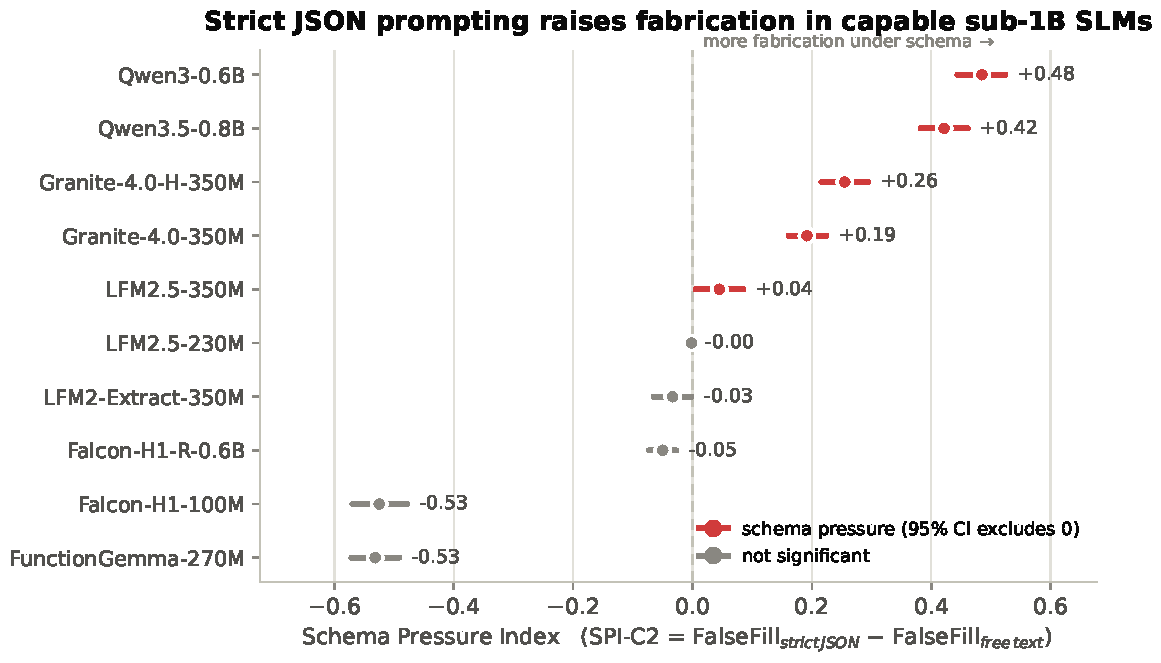
\includegraphics[width=0.92\textwidth]{figures/fig1_schema_pressure_index.pdf}
\caption{\spi-C2 with 95\% bootstrap confidence intervals. Positive values mean strict JSON increased false filling compared with free text extraction.}
\label{fig:spi}
\end{figure}

\subsection{Explicit Null Rules Work Better than Few-Shot Null Examples}

C3 adds a direct policy: use \cnull when a value is missing, ambiguous, or contradictory. This reduces the main effect for most models. Qwen3-0.6B moves from C2 FFR 0.702 to C3 FFR 0.072. Granite-4.0-350M moves from 0.812 to 0.478, and Granite-4.0-H-350M moves from 0.645 to 0.382. Qwen3.5-0.8B remains a partial failure case: its C3 FFR is 0.440, still above its C0 FFR of 0.287, yielding a positive \spi-C3 of +0.153.

C4, the few-shot null condition, is less reliable. It improves over C3 for LFM2.5-230M, LFM2.5-350M, LFM2-350M-Extract, Qwen3.5-0.8B, and Falcon-H1-100M. It is worse than C3 for Qwen3-0.6B, both Granite models, FunctionGemma-270M, and the Falcon-H1 reasoning model. The strongest example is Qwen3-0.6B: FFR rises from 0.072 in C3 to 0.533 in C4. This refutes the planned hypothesis that few-shot null examples would consistently beat an explicit rule.

\subsection{Constrained Decoding Fixes the Object, Not the Values}

C5 tests whether schema-constrained decoding closes the gap between structure and truth. It does not. As Table~\ref{tab:c5} shows, all compatible models reach 1.00 JSON parse rate and 1.00 schema validity. False fill rates remain high for several models: LFM2.5-350M at 0.730, FunctionGemma-270M at 0.718, LFM2.5-230M at 0.717, and LFM2-350M-Extract at 0.692. The result is clearest in this condition because parsing and key/type validity are held constant.

\begin{table}[t]
\centering
\caption{C5 constrained decoding. The schema is always satisfied for compatible models, but unsupported field filling remains. Qwen3.5-0.8B is omitted because C5 was not compatible with the VLM text-only stack.}
\label{tab:c5}
\small
\begin{tabular}{@{}lcccc@{}}
\toprule
Model & Parse & Schema & FFR & Field faithfulness \\
\midrule
LFM2.5-350M & 1.000 & 1.000 & 0.730 & 0.911 \\
FunctionGemma-270M & 1.000 & 1.000 & 0.718 & 0.857 \\
LFM2.5-230M & 1.000 & 1.000 & 0.717 & 0.895 \\
LFM2-350M-Extract & 1.000 & 1.000 & 0.692 & 0.893 \\
Granite-4.0-350M & 1.000 & 1.000 & 0.480 & 0.941 \\
Falcon-H1-100M & 1.000 & 1.000 & 0.435 & 0.413 \\
Granite-4.0-H-350M & 1.000 & 1.000 & 0.297 & 0.820 \\
Falcon-H1-R-0.6B & 1.000 & 1.000 & 0.083 & 0.741 \\
Qwen3-0.6B & 1.000 & 1.000 & 0.072 & 0.781 \\
\bottomrule
\end{tabular}
\end{table}

Figure~\ref{fig:c5} plots the C5 format-truth gap. Since schema validity is fixed at 1.00, the gap is driven entirely by field errors. Falcon-H1-100M is an extreme case: it emits valid objects under C5, but field faithfulness is only 0.413.

\begin{figure}[t]
\centering
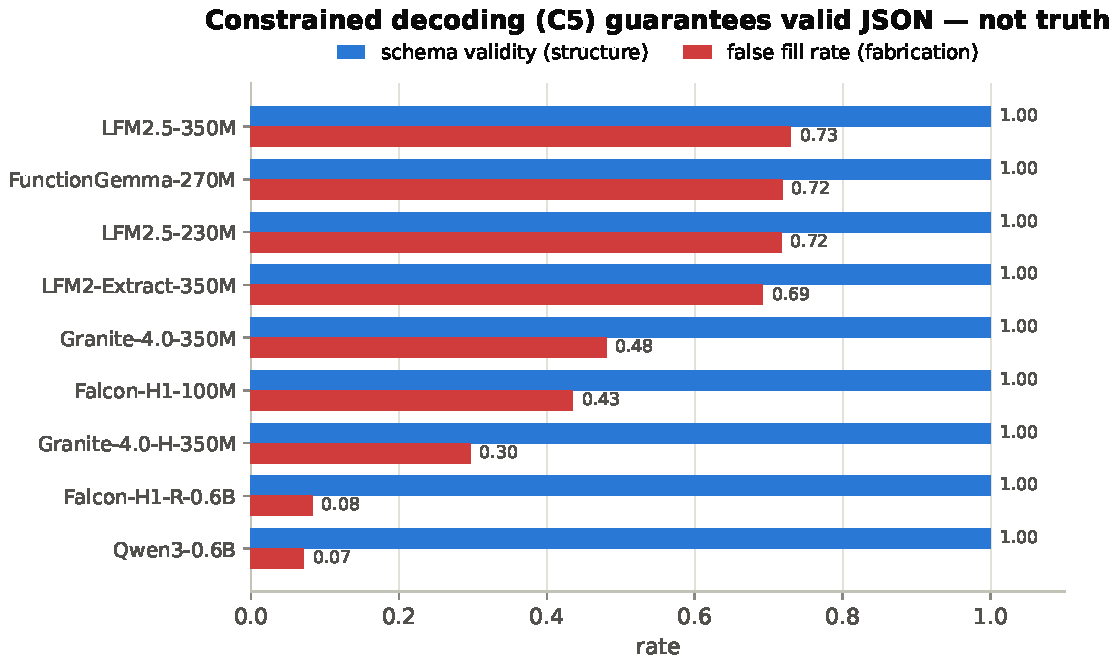
\includegraphics[width=0.85\textwidth]{figures/fig3_c5_format_truth_gap.pdf}
\caption{C5 format-truth gap. Constrained decoding gives parseable, schema-valid JSON for every compatible model, but field level correctness varies widely.}
\label{fig:c5}
\end{figure}

\subsection{Challenge Type Errors}

Averaged across the ten primary models, contradictory and ambiguous fields are hardest under C2: false fill rates are 0.740 and 0.720, respectively. Missing fields are easier, with C2 FFR 0.185. C3 improves all three null-requiring categories, reducing missing-field FFR to 0.072, ambiguous-field FFR to 0.476, and contradictory-field FFR to 0.425. Distractor copying is uncommon in this benchmark: mean distractor error is 0.002 in C2 and 0.003 in C3.

These averages hide model-specific behavior. Qwen3-0.6B has a low C3 false fill rate but loses field faithfulness in C5. LFM2-350M-Extract remains good at supported fields while filling null-required fields frequently. FunctionGemma has low C2 false filling only because strict JSON fails to parse.

\subsection{Sampling Replication and Quantization}

The C2 main effect replicates under stochastic decoding for the five positive models. The sampled \spi-C2 means are close to deterministic values: Qwen3-0.6B +0.487 $\pm$ 0.003, Qwen3.5-0.8B +0.398 $\pm$ 0.004, Granite-4.0-H-350M +0.249 $\pm$ 0.006, Granite-4.0-350M +0.180 $\pm$ 0.004, and LFM2.5-350M +0.063 $\pm$ 0.006. Figure~\ref{fig:replication} compares deterministic and sampled \spi-C2 values.

\begin{figure}[t]
\centering
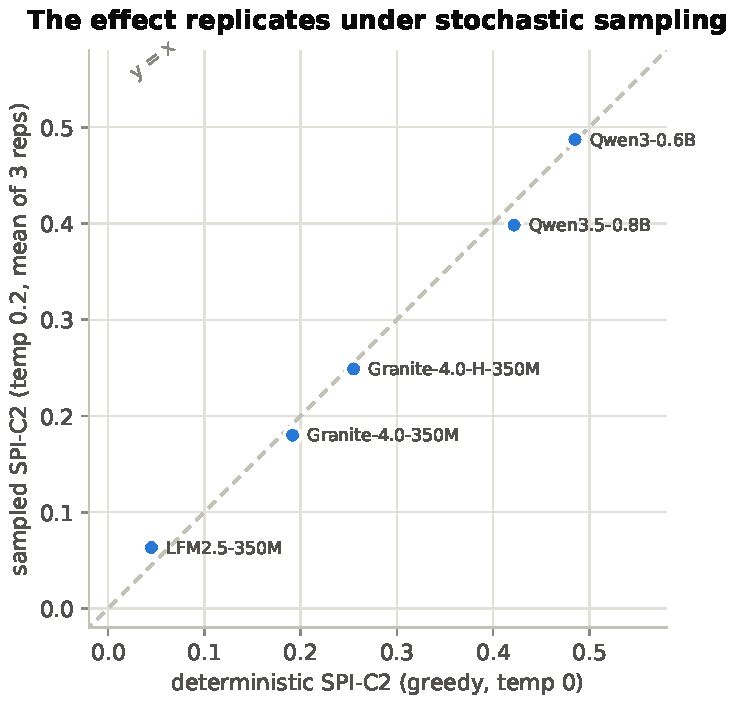
\includegraphics[width=0.78\textwidth]{figures/fig4_replication_scatter.pdf}
\caption{Sampling replication for \spi-C2. The five models with positive deterministic \spi-C2 remain positive at temperature 0.2 across three repetitions.}
\label{fig:replication}
\end{figure}

Quantization does not change the qualitative result for Qwen3-0.6B: \spi-C2 is +0.482 for INT8 and +0.492 for INT4, close to +0.485 in the main run. The LFM models are less stable. LFM2.5-350M increases from +0.045 in the main run to +0.072 under INT8 and +0.133 under INT4. LFM2.5-230M moves in the opposite direction, with negative \spi-C2 under both quantized variants. These results are best treated as deployment checks, not as a general claim about quantization, because only five model families were compatible with the quantization pass.

\subsection{Qualitative Examples}

Table~\ref{tab:qual} gives three representative false fills. The first two are classic schema pressure errors: the model supplies a plausible event name even though the title is explicitly unspecified. The third is a type and field error: a date is copied into an age slot. All three outputs are parseable JSON; two pass schema validation.

\begin{table}[t]
\centering
\caption{Representative false fill errors. Gold \cnull means the field should have been left empty.}
\label{tab:qual}
\small
\begin{tabularx}{\textwidth}{@{}l l X l@{}}
\toprule
Model & Field & Context evidence & Model value \\
\midrule
Qwen3-0.6B, C2 & event & activity title was not specified & ``general after-school activity'' \\
Qwen3.5-0.8B, C2 & event & activity title was not specified & ``general after-school activity'' \\
Granite-4.0-350M, C2 & age & age was not stated & ``2026-02-08'' \\
\bottomrule
\end{tabularx}
\end{table}

\section{Discussion}

The experiments support a bounded version of the schema pressure hypothesis. Strict JSON prompting can increase unsupported field completion, but the effect depends on the base model. The models that are both capable of producing strict JSON and not already at a free text false fill ceiling show the clearest increases. Models that fail structurally can appear safe on false fill metrics unless parse and schema validity rates are reported beside them.

This leads to a practical rule for evaluating sub-1B structured output systems: never report JSON validity alone. C5 makes this point directly. A constrained decoder can force every key and every type while leaving unsupported-value behavior unchanged or only partly improved. The field value must still be evaluated against evidence.

The mitigation result is also useful. The explicit null rule is simple, cheap, and often effective. Few-shot examples are not a drop-in replacement. In this experiment, few-shot null examples helped some LFM models and Qwen3.5, but hurt Qwen3-0.6B and the Granite models. A likely reason is that few-shot prompts change more than the abstention policy: they lengthen the prompt, add a local style, and may shift the model toward copying example structure in ways that interact with its instruction tuning. The experiment does not prove that few-shot prompting is bad; it shows that it should be validated per model rather than assumed safe.

\section{Limitations}

The benchmark is synthetic and flat. It controls evidence status well, but it does not cover long documents, nested schemas, noisy OCR, multilingual contexts, or domain-specific forms. The next version should add nested objects and real documents while preserving field level evidence labels.

The C5 constrained decoding result is framework-specific. The returned package records lm-format-enforcer for C5. Other grammar engines may differ in speed, supported schema features, or token-level behavior. The core point remains narrower: any decoding engine that only constrains syntax cannot by itself verify whether a value is supported by the source text.

The Qwen3.5-0.8B row requires care. The model is multimodal and was run through a text-only path. C5 was not available for that stack. We therefore use Qwen3-0.6B as a pure-text Qwen control rather than treating Qwen3.5 as the only Qwen result.

The planned optional-field ablation, where unsupported fields could be omitted instead of set to \cnull, was not present in the returned experiment package. This version of the paper therefore does not claim whether required keys create more pressure than optional keys. That ablation is the most direct next test of the mechanism.

Finally, exact matching is conservative. A plausible guess is still wrong unless the context supports it. This is intentional for safety-critical extraction, but it can understate usefulness in applications where approximate labels are acceptable.

\section{Conclusion}

Sub-1B models can produce outputs that are easy for software to consume. That does not make the values safe to consume. In \sass, strict JSON increases unsupported field filling for five of ten recent sub-1B models, and constrained decoding gives perfect parse and schema validity while leaving false fill rates high for several models. Explicit null instructions reduce the error more consistently than few-shot null examples. The main lesson is simple: for structured output SLMs, evaluation must score both the object and the evidence behind each field.

\section*{Artifact and Reproducibility Notes}

The submission package used for this paper contains the benchmark JSONL file, prompt templates, raw outputs, field level metrics, summary CSV files, confidence intervals, figures, and scoring scripts. The main paper uses the JSON-aware C0 fallback in \code{results/c0robust/}. The source package includes the three summary CSV files used for the main tables and confidence intervals.

\begin{thebibliography}{99}

\bibitem{mobilellm2024}
Liu, Z., Zhao, C., Iandola, F., Lai, C., Tian, Y., Fedorov, I., Xiong, Y., Chang, E., Shi, Y., Krishnamoorthi, R., Chandra, V., Lin, Y.: MobileLLM: optimizing sub-billion parameter language models for on-device use cases. In: Proceedings of the 41st International Conference on Machine Learning. Proceedings of Machine Learning Research, vol.~235 (2024). \url{https://proceedings.mlr.press/v235/liu24ce.html}

\bibitem{jsonschemabench}
Geng, S., Cooper, H., Moskal, M., Jenkins, S., Berman, J., Ranchin, N., West, R., Horvitz, E., Nori, H.: Generating structured outputs from language models: benchmark and studies. arXiv:2501.10868 (2025). \url{https://arxiv.org/abs/2501.10868}

\bibitem{abstentionbench}
Kirichenko, P., Ibrahim, M., Chaudhuri, K., Bell, S.J.: AbstentionBench: reasoning LLMs fail on unanswerable questions. arXiv:2506.09038 (2025). \url{https://arxiv.org/abs/2506.09038}

\bibitem{structuredoutputbench}
Singh, A.K., Khurdula, H.V., Khemlani, Y.D., Agarwal, V.: The Structured Output Benchmark: a multi-source benchmark for evaluating structured output quality in large language models. arXiv:2604.25359 (2026). \url{https://arxiv.org/abs/2604.25359}

\bibitem{llmstructbench}
Tenckhoff, S., Koddenbrock, M., Rodner, E.: LLMStructBench: benchmarking large language model structured data extraction. arXiv:2602.14743 (2026). \url{https://arxiv.org/abs/2602.14743}

\bibitem{qwen3tr}
Yang, A., Li, A., Yang, B., Zhang, B., Hui, B., Zheng, B., Yu, B., Gao, C., Huang, C., Lv, C., Zheng, C., Liu, D., Zhou, F., Huang, F., Hu, F., Ge, H., Wei, H., Lin, H., Tang, J., Yang, J., et al.: Qwen3 technical report. arXiv:2505.09388 (2025). \url{https://arxiv.org/abs/2505.09388}

\bibitem{falconh1}
Zuo, J., Velikanov, M., Chahed, I., Belkada, Y., Rhayem, D.E., Kunsch, G., Hacid, H., Yous, H., Farhat, B., Khadraoui, I., Farooq, M., Campesan, G., Cojocaru, R., Djilali, Y., Hu, S., Chaabane, I., Khanna, P., Seddik, M.E.A., Huynh, N.D., Khac, P.L., et al.: Falcon-H1: a family of hybrid-head language models redefining efficiency and performance. arXiv:2507.22448 (2025). \url{https://arxiv.org/abs/2507.22448}

\bibitem{liquidlfm25}
Liquid AI: LFM2.5-230M and LFM2.5-350M model cards. Hugging Face (2026). \url{https://huggingface.co/LiquidAI/LFM2.5-230M}, \url{https://huggingface.co/LiquidAI/LFM2.5-350M}

\bibitem{liquidextract}
Liquid AI: LFM2-350M-Extract model card. Hugging Face (2026). \url{https://huggingface.co/LiquidAI/LFM2-350M-Extract}

\bibitem{qwen35hf}
Qwen Team: Qwen3.5-0.8B model card. Hugging Face (2026). \url{https://huggingface.co/Qwen/Qwen3.5-0.8B}

\bibitem{qwen3hf}
Qwen Team: Qwen3-0.6B model card. Hugging Face (2026). \url{https://huggingface.co/Qwen/Qwen3-0.6B}

\bibitem{granite350}
IBM Granite Team: Granite-4.0-350M model card. Hugging Face (2026). \url{https://huggingface.co/ibm-granite/granite-4.0-350m}

\bibitem{graniteh350}
IBM Granite Team: Granite-4.0-H-350M model card. Hugging Face (2026). \url{https://huggingface.co/ibm-granite/granite-4.0-h-350m}

\bibitem{functiongemma}
Google: FunctionGemma-270M-IT model card and documentation. Hugging Face, Google AI for Developers (2026). \url{https://huggingface.co/google/functiongemma-270m-it}

\end{thebibliography}

\appendix

\section{Prompt Conditions}

The experiment used fixed templates. The main distinctions are summarized here. C0 requested line-based output and \code{UNKNOWN} for unsupported values. C1 requested JSON with the five keys. C2 required only valid JSON and exactly the five keys. C3 added: use \cnull when a value is not directly stated, ambiguous, or contradictory; do not guess. C4 prepended three examples whose correct outputs included \cnull. C5 used the C3 text with schema-constrained decoding.

\section{JSON Schema}

Every field allowed \cnull, so unsupported values were never required by the schema.
\begin{verbatim}
{
  "type": "object",
  "additionalProperties": false,
  "required": ["target_name", "target_age",
               "event_name", "city", "event_date"],
  "properties": {
    "target_name": {"type": ["string", "null"]},
    "target_age": {"type": ["integer", "null"]},
    "event_name": {"type": ["string", "null"]},
    "city": {"type": ["string", "null"]},
    "event_date": {"type": ["string", "null"]}
  }
}
\end{verbatim}

\section{Quantization Add-On}

\begin{table}[H]
\centering
\caption{Quantized variants. Positive \spi-C2 under INT8/INT4 means strict JSON raised false filling after quantization.}
\small
\begin{tabular}{@{}llccc@{}}
\toprule
Base model & Variant & FFR C0 & FFR C2 & \spi-C2 \\
\midrule
Qwen3-0.6B & INT8 & 0.230 & 0.712 & +0.482 \\
Qwen3-0.6B & INT4 & 0.192 & 0.683 & +0.492 \\
LFM2.5-350M & INT8 & 0.688 & 0.760 & +0.072 \\
LFM2.5-350M & INT4 & 0.730 & 0.863 & +0.133 \\
LFM2.5-230M & INT8 & 0.752 & 0.497 & -0.255 \\
LFM2.5-230M & INT4 & 0.745 & 0.710 & -0.035 \\
LFM2-350M-Extract & INT8 & 0.760 & 0.742 & -0.018 \\
LFM2-350M-Extract & INT4 & 0.752 & 0.787 & +0.035 \\
FunctionGemma-270M & INT8 & 0.592 & 0.000 & -0.592 \\
FunctionGemma-270M & INT4 & 0.630 & 0.002 & -0.628 \\
\bottomrule
\end{tabular}
\end{table}

\end{document}
